\subsection{iOS}
	Das Kapitel Verschlüsselung unter iOS stellt zu Beginn eingesetzte Hardware vor
	und anschließend rückt der Fokus auf die logische Ebene, mit einem zusätzlichen
	Blick auf den Dateizugriff.
	\subsubsection{Kryptographische Hardware}\label{sec:crypto-engine}
		Für eine native Verschlüsselung sorgt in jedem iOS Gerät eine 256-Bit
		basierte AES Hardware-Engine, welche zwischem dem Flash	Speicher und dem
		Systemspeicher liegt (vgl. Abb. \ref{fig:security-model}). Diese
		Positionierung sorgt für hohe Performance und niedrige Latenzen beim
		Ver- und Entschlüsseln von Dateien. Die geräteeigene Unique ID wird beim
		Herstellungsprozess in den Applikationsprozessor und den Secure Enclave
		eingebrannt und die Group ID wird compiliert, somit ist es keiner Soft- oder
		Firmware möglich diese direkt zu lesen (vgl. Kapitel
		\ref{sec:secure-boot-chain}). Dies verhindert eine Manipulation oder ein
		Umgehen dieser Schlüssel, sowie einen Zugriff außerhalb der Krypto-Engine.
		Die UID erlaubt außerdem eine gerätespezifische Bindung von Daten. Apple
		beteuert unter anderem
		\begin{quote}
			The UIDs are unique to each device and are not recorded by Apple or any of its
			suppliers \cite[S.9]{iOSSecurityApr2015}.
		\end{quote}
		Die GID hingegen ist allen Geräten einer
		Prozessorklasse bekannt, z.B.
		all jenen die einen Apple A7 nutzen. Dies liegt an der weniger
		Sicherheitskritischen Nutzung dieser Schlüssel für Vorgänge,
		wie beispielsweise die Übertragung von Systemsoftware bei Updates. Jegliche
		weitere bei Kryptografischen Operationen benötigte Schlüssel werden von einem
		Random Number Generator (RNG) mit einem auf	CTR\_DRBG \cite{NISTDRBG2012}
		basierenden Algorithmus erzeugt.
	\subsubsection{Schutz auf Dateiebene}\label{sec:filesecurity}
		Zusätzlich zur Hardwareverschlüsselung nutzt iOS ein Feature namens
		\textsl{Data Protection} um Daten im Flash Speicher zu schützen. Dieser
		Mechanismus wird bei allen System Apps und ab iOS 7 auch bei Drittanbieter Apps
		automatisch angewendet. Die Funktionsweise ist in Form einer
		Schlüsselhierarchie im Verbund mit Hardwareverschlüsselung realisiert. Jede
		Datei, die in den Speicher geschrieben wird, erhält einen 256-Bit, explizit
		ihr zugewiesenen, \textsl{Per-File} Schlüssel. Dieser wird von der
		Verschlüsselungsengine (Kapitel \ref{sec:crypto-engine}) mit Hilfe von
		AES CBC (vgl. Kapitel \ref{sec:encrypt-volume})
		verschlüsselt. Der Per-File Schlüssel wird mit einem von vier
		Klassenschlüsseln ummantelt und in den Meta-Daten gespeichert. Die vier
		möglichen Schlüssel sind:
		\begin{itemize}
		  \item \textsl{Complete Protection}: Klassenschlüssel wird mit einem
		  Schlüssel, abgeleitet aus passcode und UID, verschlüsselt. 10 Sekunden (wenn
		  die "`Passwort benötigt"' Funktion ohne Verzögerung eingestellt wurde) nach
		  Sperren des Gerätes wird dieser Schlüssel verworfen.
		  \item \textsl{Protected Unless Open}: Während das Gerät gesperrt ist, können
		  bestimmte Dateien, wie beispielsweise ein E-Mail Anhang der heruntergeladen
		  wird, dennoch geschrieben werden. Um dies zu ermöglichen wird
		  Elliptische-Kurven-Kryptographie eingesetzt (ECDH\footnote{ECDH: Elliptic
		  curve Diffie–Hellman - ein auf elliptischen Kurven basierendes
		  Schlüsselaustauschverfahren} mit Curve25519\footnote{Curve25519 - eine
		  elliptische Kurve, welche auch für Schlüsselaustauschprotokolle genutzt
		  wird}).
		  \item \textsl{Protected Until First User Authentication}: Der Unterscheid zu
		  \textsl{Complete Protection} besteht darin, dass der genutzte Schlüssel
		  beim Sperren des Gerätes nicht verworfen wird. Diese Klasse wird per
		  Standard für Drittanbieter Apps verwendet, wenn nicht explizit angepasst.
		  \item \textsl{No Protection}: Hier wird der Klassenschlüssel nur mit der UID
		  verschlüsselt und im \textsl{Effaceable
		  Storage}\footnote{Effaceable Storage - dedizierter Bereich im NAND-Speicher,
		  welcher direkt adressiert und sicher gelöscht werden kann} gespeichert.
		\end{itemize}
		Jegliche Meta-Daten sind mit einem zufälligen Schlüssel verschlüsselt, welcher
		beim installieren von iOS oder beim Löschen eines Gerätes durch den Benutzer
		erstellt wird. Beim Entschlüsseln einer Datei, werden zuerst die Meta-Daten
		mit dem \textsl{File System Key} entschlüsselt. Dieser ist im Effaceable Storage
		gespeichert.
		Sobald dieser Speicher und somit der darin enthaltene Dateisystemschlüssel
		gelöscht wurde, macht dies alle Dateien auf dem Gerät kryptografisch
		unwiederherstellbar. Wenn der Benutzer \textsl{passcode} auf dem System
		einrichtet, aktiviert er Data Protection automatisch.
		\begin{figure}[h]
			\centering
			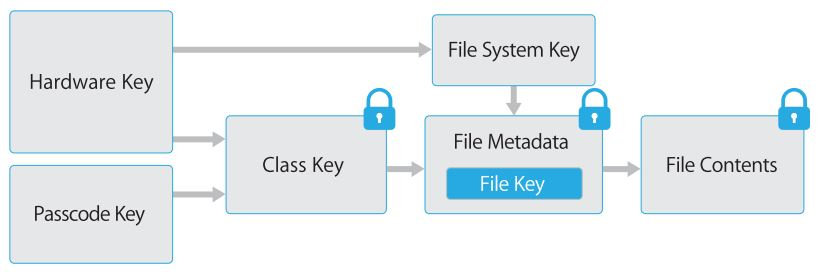
\includegraphics[width=0.9\linewidth]{ios/media/data-protection.jpg}
			\caption{Data Protection Architektur 
			\cite[S.10]{iOSSecurityApr2015}}
			\label{fig:data-protection}
		\end{figure}
